\documentclass{beamer}

% Minimal theme
\usetheme{default}

% Remove navigation symbols
\setbeamertemplate{navigation symbols}{}
\setbeamertemplate{footline}{}

% Package for including PDF pages
\usepackage{pdfpages}

% Additional packages for plots
\usepackage{pgfplots}
\usepackage{tikz}
\pgfplotsset{compat=1.18}

\title{Univariate Optimization}


\begin{document}

% Title page
\begin{frame}
\titlepage
\end{frame}

\begin{frame}
\frametitle{Content Overview}
\begin{itemize}
    \item Convex Sets / Convex Functions
    \item Unimodal Functions
    \item Univariate Optimization Methods (Golden Section Search, Brent's Method)
    \item Stopping Criteria
\end{itemize}
\end{frame}

% Include pages on local/global optimums and convex functions
\section{Convexity}

\includepdf[pages={25-29}]{slides_lmu/01_math.pdf}

% only page 33
\includepdf[pages={33}]{slides_lmu/01_math.pdf}

% ========================================
% UNIMODAL FUNCTIONS
% ========================================
\section{Unimodal Functions}

\begin{frame}
\frametitle{Unimodal Functions: Definition}
\begin{definition}
A function $f: \mathbb{R} \to \mathbb{R}$ is called \textbf{unimodal} if it has exactly one local optimum (minimum or maximum), which is also the global optimum.
\end{definition}

\vspace{0.5cm}

\textbf{Formal Definition:}
\begin{itemize}
    \item For a unimodal function with minimum at $x^*$:
    \begin{itemize}
        \item $f$ is strictly decreasing on $(-\infty, x^*]$
        \item $f$ is strictly increasing on $[x^*, \infty)$
    \end{itemize}
    \item For a unimodal function with maximum at $x^*$:
    \begin{itemize}
        \item $f$ is strictly increasing on $(-\infty, x^*]$
        \item $f$ is strictly decreasing on $[x^*, \infty)$
    \end{itemize}
\end{itemize}
\end{frame}

\begin{frame}
\frametitle{Unimodal Functions: Key Properties}
\textbf{Important Properties:}
\begin{itemize}
    \item Any local optimum is also the global optimum
    \item Optimization is easier: no risk of getting stuck in local optima
\end{itemize}

\vspace{0.5cm}

\end{frame}

\begin{frame}
\frametitle{Example 1: Quadratic Function (Convex \& Unimodal)}
\begin{columns}
\begin{column}{0.5\textwidth}
$$f(x) = x^2$$

\vspace{0.3cm}

\textbf{Properties:}
\begin{itemize}
    \item Convex
    \item Unimodal
    \item Global minimum at $x^* = 0$
    \item Strictly decreasing on $(-\infty, 0]$
    \item Strictly increasing on $[0, \infty)$
\end{itemize}
\end{column}
\begin{column}{0.5\textwidth}
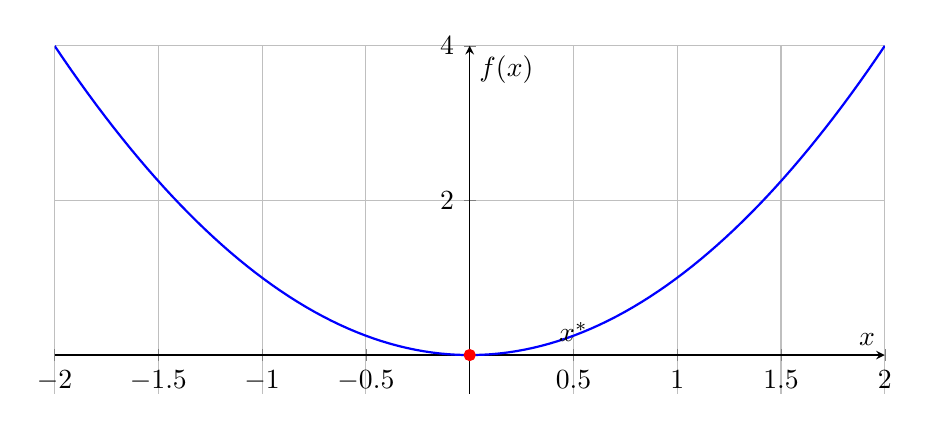
\begin{tikzpicture}
\begin{axis}[
    width=\textwidth,
    height=6cm,
    axis lines=middle,
    xlabel=$x$,
    ylabel=$f(x)$,
    domain=-2:2,
    samples=100,
    ymin=-0.5,
    ymax=4,
    grid=major,
]
\addplot[blue, thick] {x^2};
\addplot[red, mark=*, only marks] coordinates {(0,0)};
\node at (axis cs:0.5,0.3) {$x^*$};
\end{axis}
\end{tikzpicture}
\end{column}
\end{columns}
\end{frame}

\begin{frame}
\frametitle{Example 2: Absolute Value }
\begin{columns}
\begin{column}{0.5\textwidth}
$$f(x) = -|x|$$

\vspace{0.3cm}

\textbf{Properties:}
\begin{itemize}
    \item NOT convex (concave)
    \item Unimodal
    \item Global maximum at $x^* = 0$
    \item Strictly increasing on $(-\infty, 0]$
    \item Strictly decreasing on $[0, \infty)$
\end{itemize}
\end{column}
\begin{column}{0.5\textwidth}
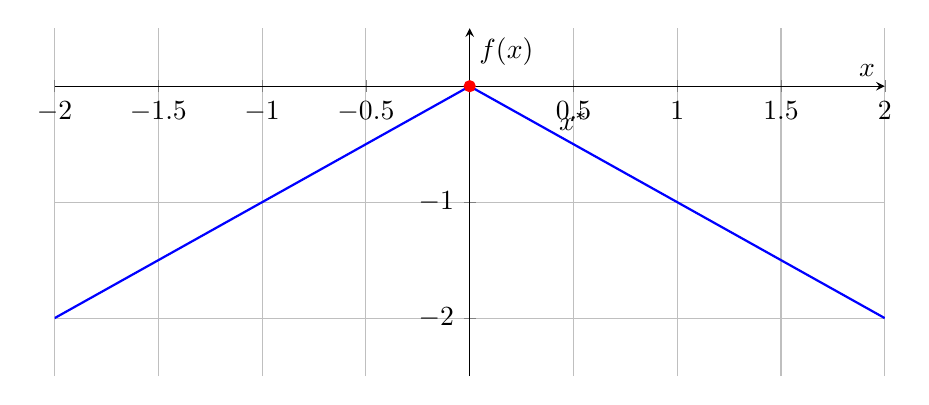
\begin{tikzpicture}
\begin{axis}[
    width=\textwidth,
    height=6cm,
    axis lines=middle,
    xlabel=$x$,
    ylabel=$f(x)$,
    domain=-2:2,
    samples=100,
    ymin=-2.5,
    ymax=0.5,
    grid=major,
]
\addplot[blue, thick] {-abs(x)};
\addplot[red, mark=*, only marks] coordinates {(0,0)};
\node at (axis cs:0.5,-0.3) {$x^*$};
\end{axis}
\end{tikzpicture}
\end{column}
\end{columns}
\end{frame}

\begin{frame}
\frametitle{Counter-Example: Non-Unimodal Function}
\begin{columns}
\begin{column}{0.5\textwidth}
$$f(x) = x^3 - 3x$$

\vspace{0.3cm}

\textbf{Properties:}
\begin{itemize}
    \item NOT unimodal
    \item Has two local optima:
    \begin{itemize}
        \item Local max at $x = -1$
        \item Local min at $x = 1$
    \end{itemize}
    \item Neither is global
    \item More challenging to optimize
\end{itemize}
\end{column}
\begin{column}{0.5\textwidth}
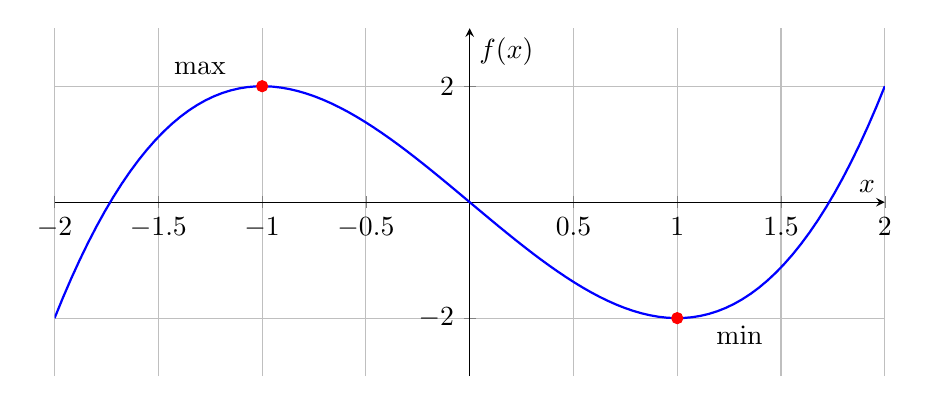
\begin{tikzpicture}
\begin{axis}[
    width=\textwidth,
    height=6cm,
    axis lines=middle,
    xlabel=$x$,
    ylabel=$f(x)$,
    domain=-2:2,
    samples=100,
    ymin=-3,
    ymax=3,
    grid=major,
]
\addplot[blue, thick] {x^3 - 3*x};
\addplot[red, mark=*, only marks] coordinates {(-1,2) (1,-2)};
\node at (axis cs:-1.3,2.3) {max};
\node at (axis cs:1.3,-2.3) {min};
\end{axis}
\end{tikzpicture}
\end{column}
\end{columns}
\end{frame}



\section{Univariate Optimization}

\begin{frame}
\frametitle{Univariate Optimization: Overview}

\textbf{Definition:} Univariate optimization involves finding the minimum or maximum of a function $f: \mathbb{R} \to \mathbb{R}$.

\textbf{Assumptions:} For algorithms discussed here, we assume that $f$ is unimodal.

\textbf{Common Methods:}
\begin{itemize}
    \item Golden Section Search
    \item Brent's Method
\end{itemize}

Golden section - \url{https://sketchplanations.com/the-golden-ratio}

Scipy optimize - \url{https://docs.scipy.org/doc/scipy/reference/optimize.html}

\end{frame}

% import entire 03_univariate file
\includepdf[pages={1-last},scale=1.35,offset=2.5cm -0.5cm]{slides_lmu/03_univariate.pdf}



% ========================================
% STOPPING CRITERIA
% ========================================
\section{Stopping Criteria}

\begin{frame}
\frametitle{Why Stopping Criteria?}
\textbf{Challenge:} Optimization algorithms are iterative and theoretically converge to the optimum as iterations $\to \infty$.

\vspace{0.5cm}

\textbf{In Practice:}
\begin{itemize}
    \item We cannot run algorithms forever
    \item Need to decide when to stop
    \item Balance between accuracy and computational cost
    \item Different criteria for different problems
\end{itemize}

\vspace{0.5cm}

\textbf{Goal:} Find a "good enough" solution in reasonable time.
\end{frame}

\begin{frame}
\frametitle{Types of Stopping Criteria}
\begin{enumerate}
    \item \textbf{Absolute Function Value Change}
    $$|f(x^{(k+1)}) - f(x^{(k)})| < \varepsilon_f$$
    
    \item \textbf{Relative Function Value Change}
    $$\frac{|f(x^{(k+1)}) - f(x^{(k)})|}{|f(x^{(k)})| + \delta} < \varepsilon_f$$
    
    \item \textbf{Absolute Parameter Change}
    $$|x^{(k+1)} - x^{(k)}| < \varepsilon_x$$
    
    \item \textbf{Gradient Norm} (if available)
    $$\|f'(x^{(k)})\| < \varepsilon_g$$
    
    \item \textbf{Maximum Iterations}
    $$k > k_{\max}$$
\end{enumerate}

\small{where $k$ is the iteration number and $\varepsilon$ values are tolerance thresholds}
\end{frame}

\begin{frame}
\frametitle{Absolute vs Relative Criteria}
\begin{columns}
\begin{column}{0.5\textwidth}
\textbf{Absolute Criteria:}
$$|f(x^{(k+1)}) - f(x^{(k)})| < \varepsilon$$

\vspace{0.3cm}
\textbf{Pros:}
\begin{itemize}
    \item Simple to implement
    \item Direct interpretation
\end{itemize}

\textbf{Cons:}
\begin{itemize}
    \item Scale-dependent
    \item Same $\varepsilon$ may be too tight for small values, too loose for large values
\end{itemize}
\end{column}

\begin{column}{0.5\textwidth}
\textbf{Relative Criteria:}
$$\frac{|f(x^{(k+1)}) - f(x^{(k)})|}{|f(x^{(k)})| + \delta} < \varepsilon$$

\vspace{0.3cm}
\textbf{Pros:}
\begin{itemize}
    \item Scale-invariant
    \item Works across different magnitudes
\end{itemize}

\textbf{Cons:}
\begin{itemize}
    \item Slightly more complex
    \item Need to handle $f(x) \approx 0$
    \item ($\delta$ is a small constant)
\end{itemize}
\end{column}
\end{columns}
\end{frame}

\begin{frame}
\frametitle{Gradient-Based Stopping Criteria}
For differentiable functions, we can use gradient information:

\vspace{0.3cm}

\textbf{First-Order Optimality Condition:}
$$\|f'(x^{(k)})\| < \varepsilon_g$$

At a local optimum: $f'(x^*) = 0$

\vspace{0.5cm}

\textbf{Advantages:}
\begin{itemize}
    \item Directly related to optimality conditions
    \item Works well near the optimum
    \item Independent of function scale (if normalized)
\end{itemize}

\vspace{0.3cm}

\textbf{Disadvantages:}
\begin{itemize}
    \item Requires gradient computation
    \item May be slow near saddle points
    \item Can give false positives at local optima
\end{itemize}
\end{frame}

\begin{frame}
\frametitle{Practical Considerations}
\textbf{Common Practice:} Use multiple criteria simultaneously
$$\text{STOP if } \begin{cases}
|f(x^{(k+1)}) - f(x^{(k)})| < \varepsilon_f & \text{AND} \\
|x^{(k+1)} - x^{(k)}| < \varepsilon_x & \text{OR} \\
k > k_{\max}
\end{cases}$$

\vspace{0.5cm}

\textbf{Typical Values:}
\begin{itemize}
    \item $\varepsilon_f = 10^{-6}$ to $10^{-8}$ (function tolerance)
    \item $\varepsilon_x = 10^{-6}$ to $10^{-8}$ (parameter tolerance)
    \item $\varepsilon_g = 10^{-5}$ to $10^{-7}$ (gradient tolerance)
    \item $k_{\max} = 100$ to $10000$ (depends on problem)
\end{itemize}

\vspace{0.3cm}

\textbf{Note:} Values depend heavily on problem scale and required precision!
\end{frame}


\end{document}
